\chapter{Утечки памяти}
\label{chap:memory-leaks}

%There are truckloads of ways for an Erlang node to bleed memory. They go from extremely simple to astonishingly hard to figure out (fortunately, the latter type is also rarer), and it's possible you'll never encounter any problem with them.
Для Erlang-узла существует огромное множество причин утечек памяти. Их выявление может оказаться как крайне простым, так и удивительно трудным (к счастью второй вид также и более редкий) и вполне вероятно, вы никогда не встретите таких проблем.

%You will find out about memory leaks in two ways:
Об утечках памяти можно узнать двумя способами:

\begin{enumerate*}
%	\item A crash dump (see Chapter \NamedRef{chap:crash-dumps});
	\item Аварийный дамп умершего узла (смотрите главу \NamedRef{chap:crash-dumps});
%	\item By finding a worrisome trend in the data you are monitoring. 
	\item Если вам удалось найти подозрительную тенденцию в изменении цифр данных, которые вы мониторите.
\end{enumerate*}

%This chapter will mostly focus on the latter kind of leak, because they're easier to investigate and see grow in real time. We will focus on finding what is growing on the node and common remediation options, handling binary leaks (they're a special case), and detecting memory fragmentation. 
Эта глава в основном сосредоточится на втором виде утечек, потому что их легче расследовать и смотреть, как они растут в реальном времени. Мы сосредоточимся на поиске того, что растёт на данном узле, обычные способы оказания первой помощи, что делать с утечками бинарных данных (они являются особым случаем), и обнаружение фрагментации памяти.


%\section{Common Sources of Leaks}
\section{Общие источники утечек}

%Whenever someone calls for help saying "oh no, my nodes are crashing", the first step is always to ask for data. Interesting questions to ask and pieces of data to consider are:
Когда кто-нибудь зовёт на помощь и говорит: <<О, нет, мои Erlang-узлы постоянно падают>>, первым дело следует попросить больше информации. Интересным будет задавать следующие вопросы и смотреть на такие подсказки:

\begin{itemize*}
%	\item Do you have a crash dump and is it complaining about memory specifically? If not, the issue may be unrelated. If so, go dig into it, it's full of data.
	\item Есть ли у вас аварийный дамп и указывает ли он конкретно на память? Если нет, проблема может быть не связана с памятью. Обязательно копните поглубже, там очень много интересного.
%	\item Are the crashes cyclical? How predictable are they? What else tends to happen at around the same time and could it be related?
	\item Являются ли падения циклическими? Насколько легко их предсказать? Что ещё происходит примерно в то же время и может повлиять на проблему?
%	\item Do crashes coincide with peaks in load on your systems, or do they seem to happen at more or less any time? Crashes that happen especially \emph{during} peak times are often due to bad overload management (see Chapter \NamedRef{chap:overload}). Crashes that happen at any time, even when load goes down following a peak are more likely to be actual memory issues.
	\item  Совпадают ли аварийные падения с всплесками нагрузки ваших систем, или происходят ли они в разное время? Падения, происходящие особенно \emph{во время} пиковых нагрузок, часто связаны с плохой обработкой ситуаций перегрузки (смотрите главу \NamedRef{chap:overload}). Падения, происходящие в разное время, даже когда нагрузка спадает после пика, могут на самом деле являться проблемами с памятью.
\end{itemize*}

%If all of this seems to point towards a memory leak, install one of the metrics libraries mentioned in Chapter \NamedRef{chap:runtime-metrics} and/or \otpapp{recon} and get ready to dive in.\footnote{See Chapter \NamedRef{chap:connecting} if you need help to connect to a running node}
Если все признаки указывают на утечку памяти, установите в вашу систему одну из библиотек метрики, которые упоминались в главе \NamedRef{chap:runtime-metrics} и/или \otpapp{recon} и приготовьтесь нырнуть в данные.\footnote{Смотрите главу \NamedRef{chap:connecting} если вам нужны подсказки, как подключиться к работающей Erlang-системе.}.

%The first thing to look at in any of these cases is trends. Check for all types of memory using \expression{erlang:memory()} or some variant of it you have in a library or metrics system. Check for the following points:
Первое, что следует искать в любом из этих случаев --- это тренды (тенденции). Проверяйте все виды памяти, используя вызов \expression{erlang:memory()} или некий аналогичный вариант, который может иметься в библиотеке или системе сбора метрик. Смотрите на следующие моменты:

\begin{itemize*}
%	\item Is any type of memory growing faster than others?
	\item Растёт ли один из видов памяти быстрее других?
%	\item Is there any type of memory that's taking the majority of the space available?
	\item Занимает ли какой-нибудь тип памяти большую часть доступного пространства?
%	\item Is there any type of memory that never seems to go down, and always up (other than atoms)?
	\item Есть ли какой-нибудь тип памяти, который никогда заметно не уменьшает потребление и только растёт вверх (кроме атомов)? Растущий график в форме пилы тоже является тревожным.
\end{itemize*}

%Many options are available depending on the type of memory that's growing.
Имеется ряд решений зависящих от типа памяти, которая начала расти.

\subsection{Атомы}

%\emph{Don't use dynamic atoms!} Atoms go in a global table and are cached forever. Look for places where you call \function{erlang:binary\_to\_term/1} and \function{erlang:list\_to\_atom/1}, and consider switching to safer variants (\expression{erlang:binary\_to\_term(Bin, [safe])} and\newline \function{erlang:list\_to\_existing\_atom/1}).
\emph{Не создавайте атомы динамически!} Атомы сохраняются в глобальной таблице навсегда. Ищите места, где вы вызываете \function{erlang:binary\_to\_term/1} и \function{erlang:list\_to\_atom/1}, и обдумайте переключение на более безопасные варианты (\expression{erlang:binary\_to\_term(Bin, [safe])} и \function{erlang:list\_to\_existing\_atom/1}). 

%If you use the \otpapp{xmerl} library that ships with Erlang, consider open source alternatives\footnote{I don't dislike \href{https://github.com/paulgray/exml}{exml} or \href{https://github.com/willemdj/erlsom}{erlsom}} or figuring the way to add your own SAX parser that can be safe\footnote{See Ulf Wiger at \href{http://erlang.org/pipermail/erlang-questions/2013-July/074901.html}{http://erlang.org/pipermail/erlang-questions/2013-July/074901.html}}. 
Если вы использовали стандартное приложение \otpapp{xmerl} в библиотеке Erlang, продумайте возможность перехода на альтернативное решение\footnote{Я не против использования \href{https://github.com/paulgray/exml}{exml} или \href{https://github.com/willemdj/erlsom}{erlsom}} или найти способ добавить собственный SAX-парсер, который мог бы оказаться безопасным\footnote{Смотрите комментарий Ulf Wiger в рассылке \href{http://erlang.org/pipermail/erlang-questions/2013-July/074901.html}{http://erlang.org/pipermail/erlang-questions/2013-July/074901.html}}.

%If you do none of this, consider what you do to interact with the node. One specific case that bit me in production was that some of our common tools used random names to connect to nodes remotely, or generated nodes with random names that connected to each other from a central server.\footnote{This is a common approach to figuring out how to connect nodes together: have one or two central nodes with fixed names, and have every other one log to them. Connections will then propagate automatically.} Erlang node names are converted to atoms, so just having this was enough to slowly but surely exhaust space on atom tables. Make sure you generate them from a fixed set, or slowly enough that it won't be a problem in the long run.
Если вы не делали ни того ни другого, задумайтесь, как вы взаимодействуете с вашим узлом. Однажны на реальной производственной системе оказалось так, что один из инструментов для подключения к узлам использовал случайные имена, или создавал узлы со случайными именами, которые подключались друг к другу с центрального сервера\footnote{Это общепринятый подход к выяснению того, как узлы подключаются друг к другу: держите два центральных узла с известными неизменными именами и остальные к ним подключаются. Тогда взаимные переподключения узлов произойдут автоматически.}. Имена узлов Erlang превращаются в атомы, так что этого оказалось достаточно, чтобы медленно и уверенно заполнить пространство таблицы атомов. Убедитесь, что вы выбираете <<случайные>> атомы из некоторого фиксированного набора, или создаёте их достаточно медленно так, чтобы это не оказалось проблемой через какое-то время.


\subsection{Двоичные данные}

Смотрите отдельную посвящённую им секцию \NamedRef{sec:binaries}.


\subsection{Код}

%The code on an Erlang node is loaded in memory in its own area, and sits there until it is garbage collected. Only two copies of a module can coexist at one time, so looking for very large modules should be easy-ish.
Код на Erlang-узлах загружается в свою особенную зону памяти, и остаётся там до тех пор, пока сборщик мусора его не освободит. Только две копии каждого модуля могут существовать одновременно в памяти, так что поиск очень больших модулей должен быть относительно лёгким.

%If none of them stand out, look for code compiled with HiPE\footnote{\href{http://www.erlang.org/doc/man/HiPE\_app.html}{http://www.erlang.org/doc/man/HiPE\_app.html}}. HiPE code, unlike regular BEAM code, is native code and cannot be garbage collected from the VM when new versions are loaded. Memory can accumulate, usually very slowly, if many or large modules are native-compiled and loaded at run time.
Если никакой модуль не выделяется из общего ряда, поищите код, скомпилированный с включенным HiPE\footnote{\href{http://www.erlang.org/doc/man/HiPE\_app.html}{http://www.erlang.org/doc/man/HiPE\_app.html}}. HiPE-код, в отличие от обычного BEAM-кода, является машинным кодом и не может быть подхвачен сборщиком мусора, когда загружаются новые версии. Память может накапливаться, обычно медленно, если много или большие HiPE-модули загружаются во время работы программы.

%Alternatively, you may look for weird modules you didn't load yourself on the node and panic if someone got access to your system!
Как вариант, можно поискать странные модули, которые вы не загружали на узел и устроить панику, если кто-то смог получить доступ к вашей системе.


\subsection{ETS}

%ETS tables are never garbage collected, and will maintain their memory usage as long as records will be left undeleted in a table. Only removing records manually (or deleting the table) will reclaim memory.
ETS-таблицы никогда не подвергаются сборке мусора и будут сохранять имеющийся расход памяти так долго, пока в них не удаляются записи. Только удаление записей вручную (или очистка/удаление всей таблицы) может вернуть память.

%In the rare cases you're actually leaking ETS data, call the undocumented \function{ets:i()} function in the shell. It will print out information regarding number of entries (\expression{size}) and how much memory they take (\expression{mem}). Figure out if anything is bad.
В редких случаях, когда у вас действительно потекла ETS-таблица, используйте недокументированную функцию \function{ets:i()} в интерактивном интерпретаторе. Она распечатает информацию о количестве записей (\expression{size}) и сколько памяти они занимают (\expression{mem}). Попробуйте использовать эти данные для поиска чего-нибудь подозрительного.

%It's entirely possible all the data there is legit, and you're facing the difficult problem of needing to shard your data set and distribute it over many nodes. This is out of scope for this book, so best of luck to you. You can look into compression of your tables if you need to buy time, however.\footnote{See the \href{http://www.erlang.org/doc/man/ets.html\#new-2}{\expression{compressed} option for \function{ets:new/2}}}
Совершенно возможен случай, когда все данные в таблице находятся честно и согласно алгоритму вашей программы, и вы столкнулись с проблемой необходимости разделения таблицы на секции (\emph{sharding}) и распределения на разные узлы. Это выходит за пределы книги, так что удачи вам. Однако стоит посмотреть на опцию сжатия таблиц, если вам нужно выиграть время\footnote{Смотрите опцию \href{http://www.erlang.org/doc/man/ets.html\#new-2}{\expression{compressed} для \function{ets:new/2}}}.


\subsection{Процессы}

%There are a lot of different ways in which process memory can grow. Most interesting cases will be related to a few common cases: process leaks (as in, you're leaking processes), specific processes leaking their memory, and so on. It's possible there's more than one cause, so multiple metrics are worth investigating. Note that the process count itself is skipped and has been covered before.
Есть множество разных причин роста памяти процессов. Самые интересные случаи относятся к нескольким самым частым причинам: утечки процессов (то есть, течёт не память, а теряются целые процессы), утечки памяти в особых процессах, и так далее. Возможно в вашем случае будет более одной причины одновременно, так что смотрите сразу на многие метрики. Заметьте, что счёт процессов был описан ранее и поэтому на нём здесь не останавливаемся.


%\subsubsection{Links and Monitors}
\subsubsection{Связи и мониторы}

%Is the global process count indicative of a leak? If so, you may need to investigate unlinked processes, or peek inside supervisors' children lists to see what may be weird-looking.
Является ли глобальное количество процессов индикатором утечки? Если так, то вам может понадобиться рассмотреть процессы, с которыми была разорвана связь (\emph{unlinked}), или заглянуть в списки дочерних процессов наблюдателей на случай, если они выглядят необычно.

%Finding unlinked (and unmonitored) processes is easy to do with a few basic commands:
Поиск процессов, с которыми была разорвана связь и мониторинг --- это несложная задача при помощи нескольких простых команд.

\begin{VerbatimEshell}
1> [P || P <- processes(),
         [{_,Ls},{_,Ms}] <- [process_info(P, [links,monitors])],
         []==Ls, []==Ms].
\end{VerbatimEshell}

%This will return a list of processes with neither. For supervisors, just fetching \newline \expression{supervisor:count\_children(SupervisorPidOrName)} and seeing what looks normal can be a good pointer.
Эта команда вернёт список процессов не имеющих ни того ни другого. Для наблюдателей хорошей подсказкой может быть простая выборка с помощью \expression{supervisor:count\_children(SupervisorPidOrName)} и проверка на глаз: выглядит ли список хорошо или подозрительно.


%\subsubsection{Memory Used}
\subsubsection{Использованная память}

%The per-process memory model is briefly described in Subsection \NamedRef{subsec:memory-process-level}, but generally speaking, you can find which individual processes use the most memory by looking for their \term{memory} attribute. You can look things up either as absolute terms or as a sliding window.
Модель памяти с отдельной кучей для каждого процесса коротко описана в подсекции \NamedRef{subsec:memory-process-level}, но в общих словах вы можете найти конкретный процесс, использующий больше всех памяти, если посмотрите на атрибут \term{memory}. Можно смотреть за абсолютными значениями или за их изменением в скользящем интервале.

%For memory leaks, unless you're in a predictable fast increase, absolute values are usually those worth digging into first:
Для утечек памяти, если только у вас нет предсказуемого быстрого роста, стоит копнуть первым делом абсолютные значения:

\begin{VerbatimEshell}
1> recon:proc_count(memory, 3).
[{<0.175.0>,325276504,
  [myapp_stats,
   {current_function,{gen_server,loop,6}},
   {initial_call,{proc_lib,init_p,5}}]},
 {<0.169.0>,73521608,
  [myapp_giant_sup,
   {current_function,{gen_server,loop,6}},
   {initial_call,{proc_lib,init_p,5}}]},
 {<0.72.0>,4193496,
  [gproc,
   {current_function,{gen_server,loop,6}},
   {initial_call,{proc_lib,init_p,5}}]}]
\end{VerbatimEshell}

%Attributes that may be interesting to check other than \term{memory} may be any other fields in Subsection \NamedRef{subsec:digging-procs}, including \term{message\_queue\_len}, but \term{memory} will usually encompass all other types.
Атрибуты, которые могут оказаться интересными для анализа, кроме \term{memory}, --- это любые другие поля описанные в подсекции \NamedRef{subsec:digging-procs}, включая \term{message\_queue\_len}, но счётчик \term{memory} обычно включает в себя все остальные типы памяти.


%\subsubsection{Garbage Collections}
\subsubsection{Утечки сборщика мусора}
\label{subsubsec:leak-gc}

%It is very well possible that a process uses lots of memory, but only for short periods of time. For long-lived nodes with a large overhead for operations, this is usually not a problem, but whenever memory starts being scarce, such spiky behaviour might be something you want to get rid of.
Очень возможна ситуация, что процесс использует много памяти, но лишь в течение коротких промежутков времени. Для долгоживущих узлов с большими накладными расходами на выполнение работы это обычно не является проблемой, но когда ресурсы памяти становятся ограничены, то вы можете начать обдумывать план избавления от такого поведения.

%Monitoring all garbage collections in real-time from the shell would be costly. Instead, setting up Erlang's system monitor\footnote{\href{http://www.erlang.org/doc/man/erlang.html\#system\_monitor-2}{http://www.erlang.org/doc/man/erlang.html\#system\_monitor-2}} might be the best way to go at it.
Мониторинг всех сборок мусора в реальном времени из консоли интерпретатора может оказаться дорогим удовольствием. Вместо этого лучшим из решений может оказаться установка системного монитора Erlang\footnote{\href{http://www.erlang.org/doc/man/erlang.html\#system\_monitor-2}{http://www.erlang.org/doc/man/erlang.html\#system\_monitor-2}}.

%Erlang's system monitor will allow you to track information such as long garbage collection periods and large process heaps, among other things. A monitor can temporarily be set up as follows:
Системный монитор позволит вам отслеживать такую информацию, как долгие периоды сборки мусора и большие кучи процессов, а также и другие интересные вещи. Монитор можно временно запустить такими командами:

\begin{VerbatimEshell}
1> erlang:system_monitor().
undefined
2> erlang:system_monitor(self(), [{long_gc, 500}]).
undefined
3> flush().
Shell got {monitor,<4683.31798.0>,long_gc,
                   [{timeout,515},
                    {old_heap_block_size,0},
                    {heap_block_size,75113},
                    {mbuf_size,0},
                    {stack_size,19},
                    {old_heap_size,0},
                    {heap_size,33878}]}
5> erlang:system_monitor(undefined).
{<0.26706.4961>,[{long_gc,500}]}
6> erlang:system_monitor().
undefined
\end{VerbatimEshell}

%The first command checks that nothing (or nobody else) is using a system monitor yet — you don't want to take this away from an existing application or coworker.
Первая команда проверяет, что ничего (или никто) ещё не начал использовать системный монитор --- вам не хотелось бы забрать его у существующего приложения или испортить работу сотруднику.

%The second command will be notified every time a garbage collection takes over 500 milliseconds. The result is flushed in the third command. Feel free to also check for \expression{\{large\_heap, NumWords\}} if you want to monitor such sizes.
Вторая команда включает режим отправки уведомлений каждый раз, когда сборка мусора занимает дольше 500 миллисекунд. Результат можно увидеть с помощью третьей команды (которая принимает сообщения, пришедшие в процесс интерактивного интерпретатора). Попробуйте также добавить \expression{\{large\_heap, КоличествоСлов\}}, если вам интересна ситуация роста размера кучи более заданного количества слов.
%Be careful to start with large values at first if you're unsure. You don't want to flood your process' mailbox with a bunch of heaps that are 1-word large or more, for example.
Будьте осторожнее с запуском и пробуйте сначала большие значения, если не уверены в том, какие числа выбрать. Вы не хотите затопить почтовый ящик своего процесса сообщениями о том, что все кучи на узле имеют размер больше 1 слова.

%Command 5 unsets the system monitor (exiting or killing the monitor process also frees it up), and command 6 validates that everything worked.
Команда 5 отключает системный монитор (выход или смерть процесса монитора тоже его отключит) и команда 6 проверяет, что всё сработало.

%You can then find out if such monitoring messages tend to coincide with the memory increases that seem to result in leaks or overuses, and try to catch culprits before things are too bad. Quickly reacting and digging into the process (possibly with \function{recon:info/1}) may help find out what's wrong with the application.
Вы можете затем выяснить, совпадают ли подобные сообщения монитора с увеличениями размеров памяти, которые по видимости приводят к утечкам или перерасходу, и попробовать найти причину до того, как всё станет слишком плохо. Быстрое реагирование и раскопки информации по процессу (возможно с помощью \function{recon:info/1}) могут помочь выяснить, что не так с приложением.


\subsection{Ничего особенного}
%\subsection{Nothing in Particular}

%If nothing seems to stand out in the preceding material, binary leaks (Section \NamedRef{sec:binaries}) and memory fragmentation (Section \NamedRef{sec:memory-fragmentation}) may be the culprits. If nothing there fits either, it's possible a C driver, NIF, or even the VM itself is leaking. Of course, a possible scenario is that load on the node and memory usage were proportional, and nothing specifically ended up being leaky or modified. The system just needs more resources or nodes.
Если ничего из предыдущего материала не привлекло вашего внимания, то причиной могут быть утечки памяти двоичных данных (секция \NamedRef{sec:binaries}) и фрагментация памяти (секция \NamedRef{sec:memory-fragmentation}). Если даже это подозрение не оправдалось, то вполне возможно причиной является С-драйвер, встроенная (NIF) функция или даже сама виртуальная машина. Конечно, возможным сценарием может быть и то, что нагрузка на узле и расход памяти были пропорциональны, и ничего на самом деле не утекало, а расходовалось в результате нормальной работы. Системе просто требуются больше памяти или новые узлы.

%\section{Binaries}
\section{Двоичные данные}
\label{sec:binaries}

%Erlang's binaries are of two main types: ProcBins and Refc binaries\footnote{\href{http://www.erlang.org/doc/efficiency\_guide/binaryhandling.html\#id65798}{http://www.erlang.org/doc/efficiency\_guide/binaryhandling.html\#id65798}}. Binaries up to 64 bytes are allocated directly on the process's heap, and their entire life cycle is spent in there. Binaries bigger than that get allocated in a global heap for binaries only, and each process to use one holds a local reference to it in its local heap. These binaries are reference-counted, and the deallocation will occur only once all references are garbage-collected from all processes that pointed to a specific binary.
Двоичные данные в Erlang на низком уровне делятся на два вида: значения на куче процесса (\emph{ProcBin}) и большие данные в двоичной куче, освобождаемые автоматически с подсчётом ссылок (\emph{Refc})\footnote{\href{http://www.erlang.org/doc/efficiency\_guide/binaryhandling.html\#id65798}{http://www.erlang.org/doc/efficiency\_guide/binaryhandling.html\#id65798}}. Двоичные значения короче 64 байтов располагаются непосредственно в куче процесса и весь их жизненный цикл протекает там же. Двоичные значения большого размера размещаются в глобальной куче, предназначенной только для двоичных данных, и каждый процесс, который использует блок данных, хранит ссылку на него в своей локальной куче. Эти блоки данных освобождаются автоматически только тогда, когда все ссылки на них очищены сборщиком мусора во всех процессах, которые когда-либо ссылались на это значение.

%In 99\% of the cases, this mechanism works entirely fine. In some cases, however, the process will either:
Этот механизм работает совершенно удовлетворительно в 99\% случаев. Однако в некоторых ситуациях процесс может:

\begin{enumerate*}
%	\item do too little work to warrant allocations and garbage collection;
	\item выполнять слишком мало работы, чтобы оправдать выделение памяти и сборку мусора; 
%	\item eventually grow a large stack or heap with various data structures, collect them, then get to work with a lot of refc binaries. Filling the heap again with binaries (even though a virtual heap is used to account for the refc binaries' real size) may take a lot of time, giving long delays between garbage collections.
	\item вырастить большой стек или кучу с разными структурами данных, собрать их сборщиком, и затем заняться работой с большими двоичными данными. Повторное заполнение кучи такими блоками данных (даже несмотря на то, что для учёта реального размера таких блоков используется виртуальная куча) может занять долгое время, давая большие задержки между сборками мусора, соответственно и освобождение этой памяти будет отложено на будущее.
\end{enumerate*}

%\subsection{Detecting Leaks}
\subsection{Обнаружение утечек}

%Detecting leaks for reference-counted binaries is easy enough: take a measure of all of each process' list of binary references (using the \expression{binary} attribute), force a global garbage collection, take another snapshot, and calculate the difference.
Обнаружить утечку блоков двоичных данных, которые освобождаются по счётчику ссылок (\emph{refc}), довольно просто: измерьте все ссылки на двоичные данные во всех процессах (используя атрибут \expression{binary}), выполните глобальную сборку мусора, сделайте снимок ещё раз и подсчитайте разницу.

%This can be done directly with \function{recon:bin\_leak(Max)} and looking at the node's total memory before and after the call:
Это можно непосредственно выполнить с помощью функции \function{recon:bin\_leak(Количество)} и затем сравнить общую память на узле до и после вызова:

\begin{VerbatimEshell}
1> recon:bin_leak(5).
[{<0.4612.0>,-5580,
  [{current_function,{gen_fsm,loop,7}},
   {initial_call,{proc_lib,init_p,5}}]},
 {<0.17479.0>,-3724,
  [{current_function,{gen_fsm,loop,7}},
   {initial_call,{proc_lib,init_p,5}}]},
 {<0.31798.0>,-3648,
  [{current_function,{gen_fsm,loop,7}},
   {initial_call,{proc_lib,init_p,5}}]},
 {<0.31797.0>,-3266,
  [{current_function,{gen,do_call,4}},
   {initial_call,{proc_lib,init_p,5}}]},
 {<0.22711.1>,-2532,
  [{current_function,{gen_fsm,loop,7}},
   {initial_call,{proc_lib,init_p,5}}]}]
\end{VerbatimEshell}

%This will show how many individual binaries were held and then freed by each process as a delta. The value \expression{-5580} means there were 5580 fewer refc binaries after the call than before.
Это покажет нам, сколько отдельных блоков двоичных данных были заняты и затем освобождены каждым процессов в виде разности. Значение \expression{-5580} означает, что после вызова стало на 5580 меньше блоков двоичных данных (\emph{refc}), счётчики ссылок которых обнулились после первой сборки мусора.

%It is normal to have a given amount of them stored at any point in time, and not all numbers are a sign that something is bad. If you see the memory used by the VM go down drastically after running this call, you may have had a lot of idling refc binaries.
Вполне обычная ситуация иметь некоторое их количество в любой момент времени, и не любое уменьшение их количества указывает на наличие проблем. Если вы увидите, что использованная виртуальной машиной память сильно уменьшилась после вызова этой команты, у вас было значительное количество блоков двоичных данных, ссылки на которые удерживались <<спящими>> процессами.

%Similarly, if you instead see some processes hold impressively large numbers of them\footnote{We've seen some processes hold hundreds of thousands of them during leak investigations at Heroku!}, that might be a good sign you have a problem.
Подобно этому, если вы увидите, что некоторые процессы удерживают впечатляюще большие их количества\footnote{Во время наших расследований утечек памяти в Heroku мы видели процессы, удерживавшие сотни тысяч блоков памяти!}, это может быть верным знаком наличия у вас проблемы.

%You can further validate the top consumers in total binary memory by using the special \expression{binary\_memory} attribute supported in \otpapp{recon}:
Вы можете продолжить поиск самых активных пользователей блоков двоичной памяти, используя специальный атрибут \expression{binary\_memory}, который поддерживается в \otpapp{recon}:

\begin{VerbatimEshell}
1> recon:proc_count(binary_memory, 3).
[{<0.169.0>,77301349,
  [app_sup,
   {current_function,{gen_server,loop,6}},
   {initial_call,{proc_lib,init_p,5}}]},
 {<0.21928.1>,9733935,
  [{current_function,{erlang,hibernate,3}},
   {initial_call,{proc_lib,init_p,5}}]},
 {<0.12386.1172>,7208179,
  [{current_function,{erlang,hibernate,3}},
   {initial_call,{proc_lib,init_p,5}}]}]
\end{VerbatimEshell}

%This will return the \var{N} top processes sorted by the amount of memory the refc binaries reference to hold, and can help point to specific processes that hold a few large binaries, instead of their raw amount. You may want to try running this function \emph{before} \function{recon:bin\_leak/1}, given the latter garbage collects the entire node first.
Эта команда вернёт первые \var{N} процессов, отсортированные по количеству памяти, которую удерживают refc-блоки двоичных данных, и может помочь указать на конкретные процессы, владеющие небольшим количеством особо больших блоков, чего нельзя было бы увидеть, если бы вы анализировали только их количество. Вы можете решить выполнить эту функцию \emph{до} \function{recon:bin\_leak/1}, поскольку она соберёт мусор на всём узле и это повлияет на результаты.


%\subsection{Fixing Leaks}
\subsection{Исправляем утечки}

%Once you've established you've got a binary memory leak using \function{recon:bin\_leak(Max)}, it should be simple enough to look at the top processes and see what they are and what kind of work they do.
Когда вы установили факт, что у вас течёт память двоичных данных (\emph{refc}) с помощью \function{recon:bin\_leak(Количество)}, будет несложно посмотреть первые из процессов в списке и разобраться, кто они и какую работу выполняют.

%Generally, refc binaries memory leaks can be solved in a few different ways, depending on the source:
В общих словах, утечки памяти двоичных данных решаются несколькими способами в зависимости от источника проблем:

\begin{itemize*}
%	\item call garbage collection manually at given intervals (icky, but somewhat efficient);
	\item вызывать сборку мусора вручную с заданной периодичностью (неуклюжее решение, но в целом довольно эффективное);
%	\item stop using binaries (often not desirable);
	\item перестать пользоваться большими двоичными данными в целом (часто неподходящее решение);
%	\item use \function{binary:copy/1-2}\footnote{\href{http://www.erlang.org/doc/man/binary.html\#copy-1}{http://www.erlang.org/doc/man/binary.html\#copy-1}} if keeping only a small fragment (usually less than 64 bytes) of a larger binary;\footnote{It might be worth copying even a larger fragment of a refc binary. For example, copying 10 megabytes off a 2 gigabytes binary should be worth the short-term overhead if it allows the 2 gigabytes binary to be garbage-collected while keeping the smaller fragment longer.}
	\item использовать копирование с помощью \function{binary:copy/1-2}\footnote{\href{http://www.erlang.org/doc/man/binary.html\#copy-1}{http://www.erlang.org/doc/man/binary.html\#copy-1}} если требуется хранение небольшого фрагмента (обычно короче, чем 64 байта) от большого блока данных\footnote{Идея скопировать и более длинный фрагмент двоичных refc-данных может оказаться разумной. Например, копирование 10 мегабайт из 2-гигабайтового блока данных стоит своей небольшой цены, поскольку позволяет освободить 2-гигабайтовый блок в то время, как более короткий фрагмент будет нужен вам долгое время.};
%	\item move work that involves larger binaries to temporary one-off processes that will die when they're done (a lesser form of manual GC!);
	\item перенести работу, задействующую большие двоичные данные во временные процессы, которые умрут сами по завершении работы (некая упрощённая форма сборки мусора вручную);
%	\item or add hibernation calls when appropriate (possibly the cleanest solution for inactive processes).
	\item добавить вызовы спящего режима (\emph{hibernate}) там, где это имеет смысл (для часто спящих процессов --- это самый лучший подход).
\end{itemize*}

%The first two options are frankly not agreeable and should not be attempted before all else failed. The last three options are usually the best ones to be used.
Первые два варианта, честно говоря, можно считать крайними случаями и не следует пытаться их выполнять до того, как вы попробовали другие варианты. А вот последние три варианта обычно самые подходящие.


%\subsubsection{Routing Binaries}
\subsubsection{Маршрутизация двоичных данных}

%There's a specific solution for a specific use case some Erlang users have reported. The problematic use case is usually having a middleman process routing binaries from one process to another one. That middleman process will therefore acquire a reference to every binary passing through it and risks being a common major source of refc binaries leaks.
Есть одно особое решение для одного специального случая, о котором сообщали некоторые пользователи Erlang-систем. Проблемная ситуация обычно имела процесс-посредник, который маршрутизировал движение двоичных данных от одного к другому процессу. Этот процесс-посредник, таким образом, получал ссылку на каждый проходящий блок двоичных данных и рисковал оказаться основной причиной утечек или позднего освобождения двоичных данных.

%The solution to this pattern is to have the router process return the pid to route to and let the original caller move the binary around. This will make it so that only processes that do \emph{need} to touch the binaries will do so.
Решением такой ситуации является перенос работы к исполнителю --- процесс-маршрутизатор возвращал бы идентификатор процесса-получателя блока данных и вызывающий процесс передавал бы данные ему сам. Таким образом только те процессы, которым \emph{нужны} эти данные --- прикоснутся к ним и создадут ссылки на них в своих кучах.

%A fix for this can be implemented transparently in the router's API functions, without any visible change required by the callers.
В качестве решения для этого можно реализовать прозрачные функции API маршрутизатора, позволяющие изменить способ передачи данных не требуя никаких изменений в клиентах.


%\section{Memory Fragmentation}
\section{Фрагментация памяти}
\label{sec:memory-fragmentation}

%Memory fragmentation issues are intimately related to Erlang's memory model, as described in Section \NamedRef{subsec:erlang-memory-model}. It is by far one of the trickiest issues of running long-lived Erlang nodes (often when individual node uptime reaches many months), and will show up relatively rarely.
Проблемы фрагментации памяти очень близко связаны с моделью памяти Erlang, как описывалось в секции \NamedRef{subsec:erlang-memory-model}. Эта проблема --- одна из самых сложных, при эксплуатации долгоживущих Erlang-узлов (часто возникающая, когда время жизни узла достигает многих месяцев), и вы будете встречать её относительно нечасто.

%The general symptoms of memory fragmentation are large amounts of memory being allocated during peak load, and that memory not going away after the fact. The damning factor will be that the node will internally report much lower usage (through \function{erlang:memory()}) than what is reported by the operating system.
Общими симптомами фрагментации являются большие всплески распределения памяти операционной системой во время пиковой нагрузки, и то, что после спадания нагрузки память не торопится возвращаться. Смущающим фактором будет то, что внутренние отчёты виртуальной машины по памяти (\function{erlang:memory()}) будут показывать намного меньшие числа.


\subsection{Поиски фрагментации}
%\subsection{Finding Fragmentation}

%The \module{recon\_alloc} module was developed specifically to detect and help point towards the resolution of such issues.
Модуль \module{recon\_alloc} был разработан с целью помочь обнаружить и дать подсказку к решению таких проблем.

%Given how rare this type of issue has been so far over the community (or happened without the developers knowing what it was), only broad steps to detect things are defined. They're all vague and require the operator's judgement.
Зная насколько редко встречается этот тип проблем среди участников сообщества (или случался, когда разработчики не знали, что происходит), определены только широкие шаги поиска проблем. Они довольно общие и требуют оценки человеком.


%\subsubsection{Check Allocated Memory}
\subsubsection{Проверьте выделенную память}

%Calling \function{recon\_alloc:memory/1} will report various memory metrics with more flexibility than \function{erlang:memory/0}. Here are the possibly relevant arguments:
Вызов функции \function{recon\_alloc:memory/1} сообщит ряд метрик памяти в более удобном формате, чем \function{erlang:memory/0}. Вот варианты подходящих аргументов:

\begin{enumerate}
%	\item call \expression{recon\_alloc:memory(usage)}. This will return a value between 0 and 1 representing a percentage of memory that is being actively used by Erlang terms versus the memory that the Erlang VM has obtained from the OS for such purposes. If the usage is close to 100\%, you likely do not have memory fragmentation issues. You're just using a lot of it.
	\item вызовите \expression{recon\_alloc:memory(usage)}. Это вернёт значение от 0 до 1, представляющее процент активно используемой Erlang-термами памяти в сравнении с памятью, которая была взята на эти нужды у операционной системы. Если значение близко к 100\%, то, вероятно, у вас нет проблемы фрагментации, вы просто используете много памяти.
%	\item check if \expression{recon\_alloc:memory(allocated)} matches what the OS reports.\footnote{You can call \expression{recon\_alloc:set\_unit(Type)} to set the values reported by \module{recon\_alloc} in bytes, kilobytes, megabytes, or gigabytes} It should match it fairly closely if the problem is really about fragmentation or a memory leak from Erlang terms.
	\item проверьте, совпадает ли результат \expression{recon\_alloc:memory(allocated)} с числом, которое возвращает операционная система\footnote{Можно вызвать \expression{recon\_alloc:set\_unit(Единица)}, чтобы задать единицу измерения для значений, возвращаемых из \module{recon\_alloc} в байтах (bytes), килобайтах (kilobytes), мегабайтах (megabytes), или гигабайтах (gigabytes)}. Если число близко совпало, то проблема вероятно в фрагментации или утечке памяти Erlang-термов.
\end{enumerate}

%That should confirm if memory seems to be fragmented or not.
Это должно помочь укрепиться в мысли, фрагментирована ли ваша память или нет.


\subsubsection{Поиск виновного аллокатора}
%\subsubsection{Find the Guilty Allocator}

%Call \expression{recon\_alloc:memory(allocated\_types)} to see which type of util allocator (see Section \NamedRef{subsec:erlang-memory-model}) is allocating the most memory. See if one looks like an obvious culprit when you compare the results with \expression{erlang:memory()}.
Вызовите функцию \expression{recon\_alloc:memory(allocated\_types)} чтобы увидеть, какой тип вспомогательного аллокатора (смотрите секцию \NamedRef{subsec:erlang-memory-model}) выделяет больше всего памяти. Проверьте, если одно из чисел выглядит очевидным виновником, когда вы сравниваете результаты с \expression{erlang:memory()}.

%Try \expression{recon\_alloc:fragmentation(current)}. The resulting data dump will show different allocators on the node with various usage ratios.\footnote{More information is available at \href{http://ferd.github.io/recon/recon\_alloc.html}{http://ferd.github.io/recon/recon\_alloc.html}}
Попробуйте вызвать \expression{recon\_alloc:fragmentation(current)}. Распечатка данных, полученная в качестве результата, покажет различные аллокаторы на вашем узле и уровни использования ими памяти\footnote{Дополнительная информация \href{http://ferd.github.io/recon/recon\_alloc.html}{http://ferd.github.io/recon/recon\_alloc.html}}.

%If you see very low ratios, check if they differ when calling \expression{recon\_alloc:fragmentation(max)}, which should show what the usage patterns were like under your max memory load.
Если вы видите небольшие числа, то проверьте отличаются ли они, если вызвать \expression{recon\_alloc:fragmentation(max)}. Этот вызов покажет, каким было соотношение уровней при максимальной загрузке вашей памяти.

%If there is a big difference, you are likely having issues with memory fragmentation for a few specific allocator types following usage spikes.
Если вы видите большое различие, то вероятно у вас имеется проблема фрагментации для нескольких типов аллокаторов при всплеске нагрузки на узел.


%\subsection{Erlang's Memory Model}
\subsection{Модель памяти в Erlang}
\label{subsec:erlang-memory-model}

%\subsubsection{The Global Level}
\subsubsection{Взгляд снаружи}

%To understand where memory goes, one must first understand the many allocators being used. Erlang's memory model, for the entire virtual machine, is hierarchical. As shown in Figure \NamedRef{fig:allocators},  there are two main allocators, and a bunch of sub-allocators (numbered 1-9). The sub-allocators are the specific allocators used directly by Erlang code and the VM for most data types:\footnote{The complete list of where each data type lives can be found in \href{https://github.com/erlang/otp/blob/maint/erts/emulator/beam/erl\_alloc.types}{erts/emulator/beam/erl\_alloc.types}}
Чтобы понять, куда уходит память, следует сначала разобраться с множеством используемых аллокаторов. Модель памяти в Erlang, во всей виртуальной машине, организована иерархически. Как показано на рисунке \ref{fig:allocators}, имеется два основных аллокатора, которые используются из Erlang-кода и виртуальной машины для почти всех типов данных\footnote{Полный список мест, где живут разные типы данных, можно найти здесь: \href{https://github.com/erlang/otp/blob/maint/erts/emulator/beam/erl\_alloc.types}{erts/emulator/beam/erl\_alloc.types}}:


\begin{figure}
  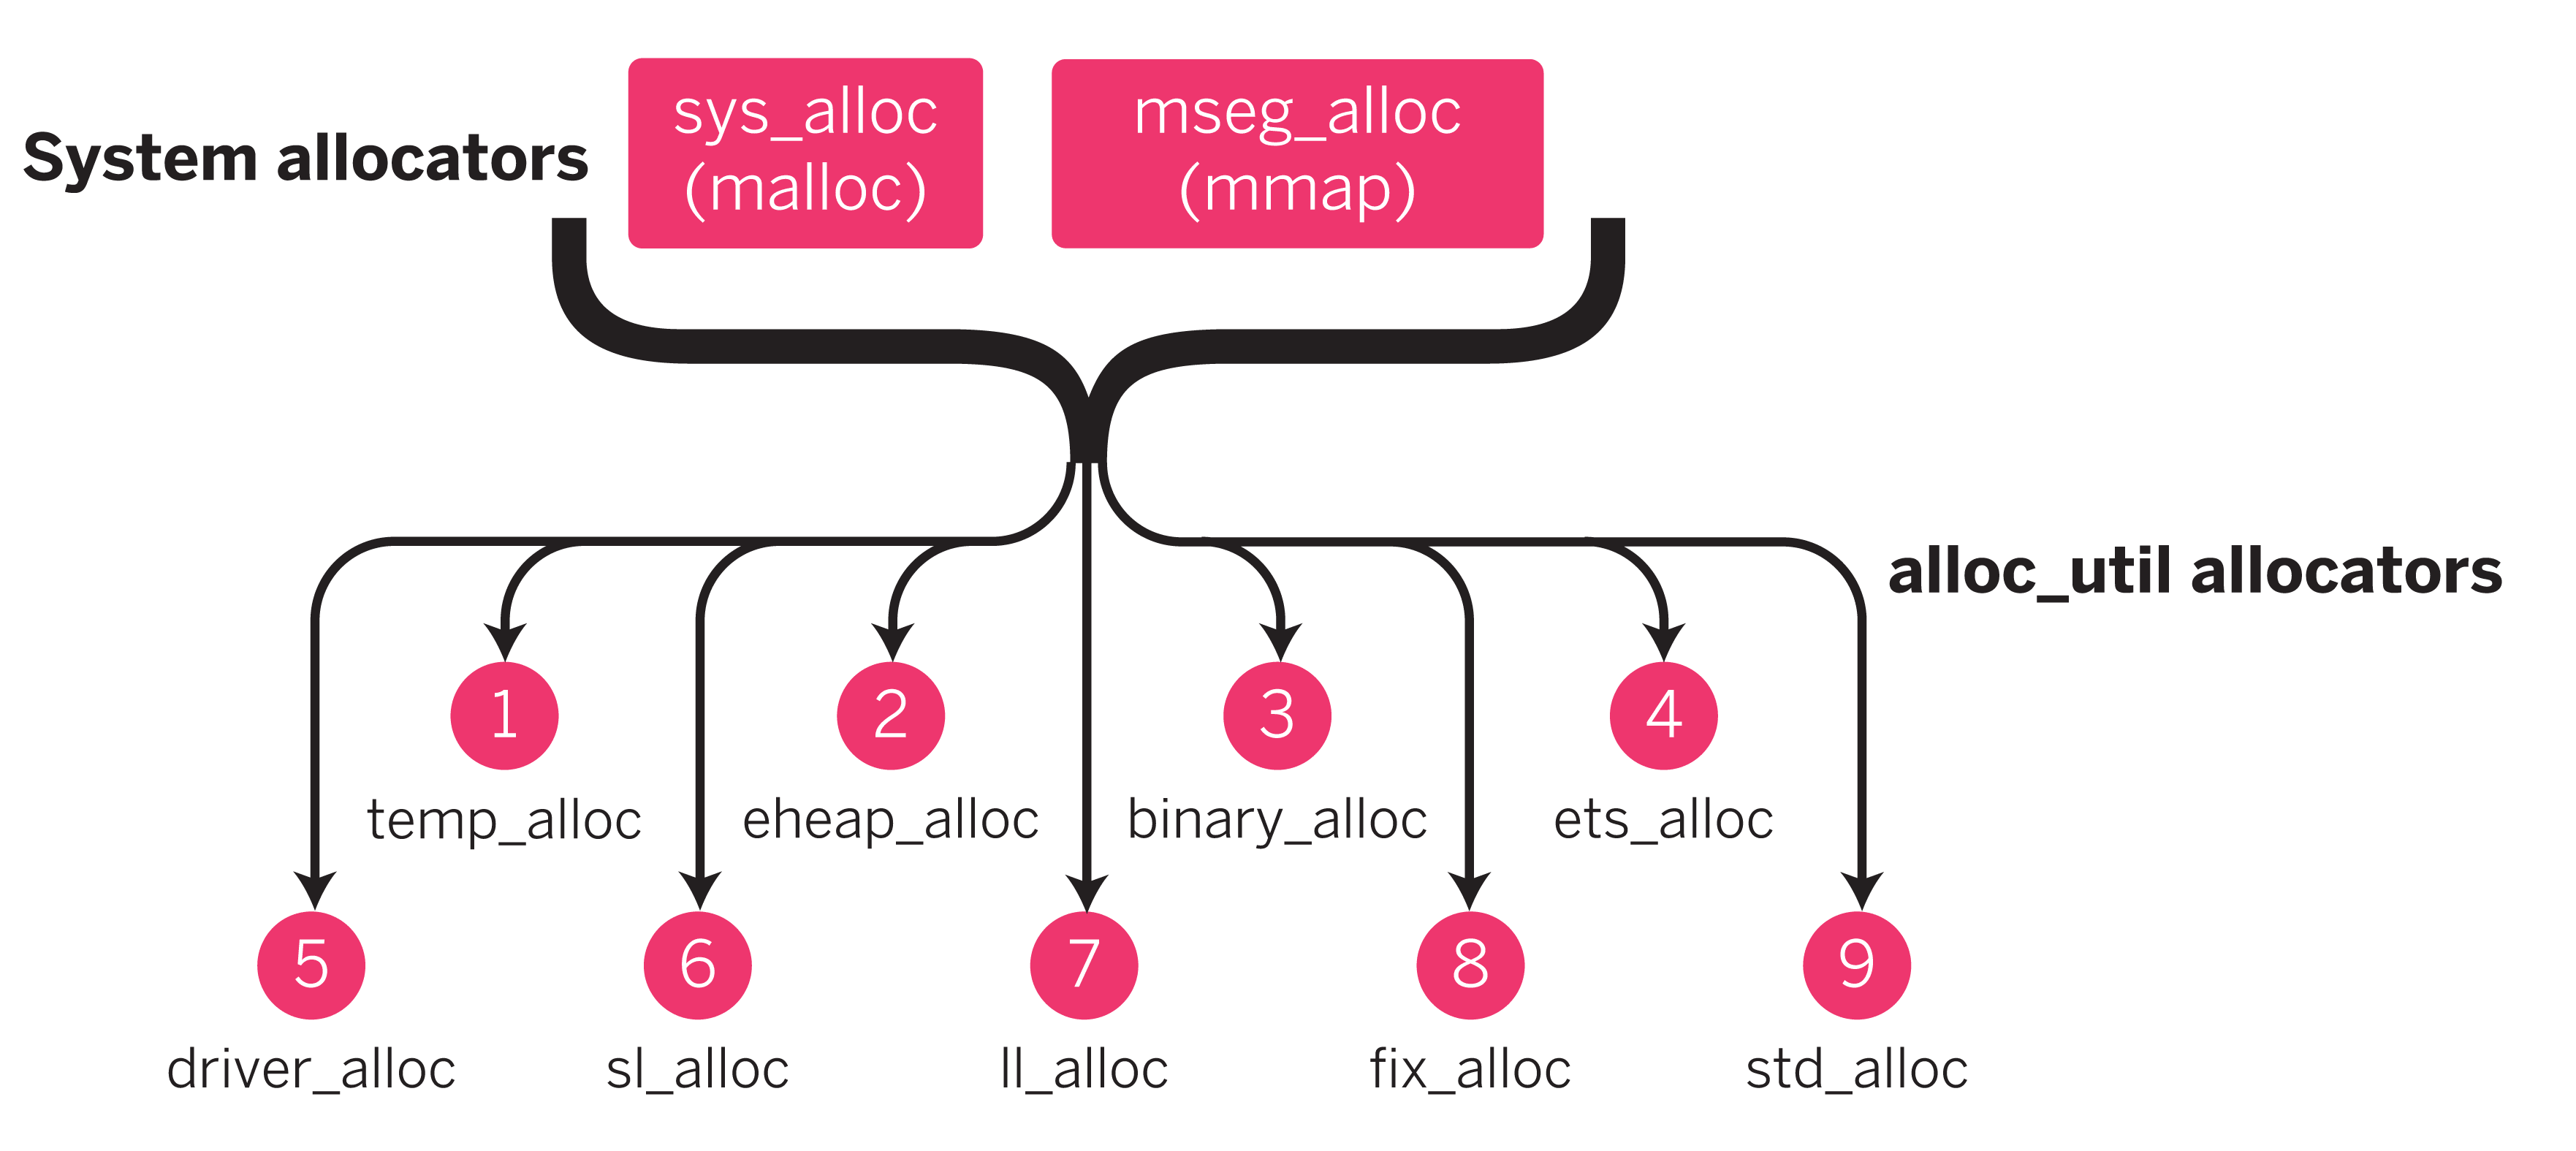
\includegraphics{memory-allocs.pdf}%
%  \caption{Erlang's Memory allocators and their hierarchy. Not shown is the special \emph{super carrier}, optionally allowing to pre-allocate (and limit) all memory available to the Erlang VM since R16B03.}%
	\caption{Аллокаторы памяти в Erlang и их иерархия. Не показаны особые \emph{супер-носители} (\emph{super carrier}), которые позволяют заранее распределять и ограничивать всю доступную память начиная с версии R16B03.}
   \label{fig:allocators}
\end{figure}

\begin{enumerate*}
%    \item \term{temp\_alloc}: does temporary allocations for short use cases (such as data living within a single C function call).
	\item \term{temp\_alloc}: выполняет временные распределения памяти для коротких задач (например, данные, живущие внутри одной С-функции).
%    \item \term{eheap\_alloc}: heap data, used for things such as the Erlang processes' heaps.
	\item \term{eheap\_alloc}: данные куч, используются для таких вещей, как кучи процессов в Erlang.
%    \item \term{binary\_alloc}: the allocator used for reference counted binaries (what their 'global heap' is). Reference counted binaries stored in an ETS table remain in this allocator.
	\item \term{binary\_alloc}: аллокатор используется для хранения двоичных данных, освобождаемых по счётчику ссылок (это их <<глобальная куча>>). Двоичные данные, хранящиеся в ETS-таблице тоже используют этот аллокатор.
%    \item \term{ets\_alloc}: ETS tables store their data in an isolated part of memory that isn't garbage collected, but allocated and deallocated as long as terms are being stored in tables.
	\item \term{ets\_alloc}: ETS-таблицы хранят свои данные в отдельной части памяти, которая не обслуживается сборщиком мусора, но живёт пока термы хранятся в таблице.
%    \item \term{driver\_alloc}: used to store driver data in particular, which doesn't keep drivers that generate Erlang terms from using other allocators. The driver data allocated here contains locks/mutexes, options, Erlang ports, etc.
	\item \term{driver\_alloc}: используется в частности для хранения данных драйверами, что впрочем не мешает им создавать Erlang-термы в других аллокаторах. Данные, выделенные здесь драйверами, могут содержать замки/мьютексы, настройки, порты Erlang и так далее.
%    \item \term{sl\_alloc}: short-lived memory blocks will be stored there, and include items such as some of the VM's scheduling information or small buffers used for some data types' handling.
	\item \term{sl\_alloc}: короткоживущие (\emph{short-lived}) блоки памяти попадают сюда и включают такие элементы, как информация планировщика виртуальной машины или маленькие буферы для нужд обработки некоторых типов данных.
%    \item \term{ll\_alloc}: long-lived allocations will be in there. Examples include Erlang code itself and the atom table, which stay there.
	\item \term{ll\_alloc}: долгоживущие (\emph{long-lived}) распределения памяти идут сюда. Примерами является сам Erlang-код и таблица атомов, которые остаются надолго.
%    \item \term{fix\_alloc}: allocator used for frequently used fixed-size blocks of memory. One example of data used there is the internal processes' C struct, used internally by the VM.
	\item \term{fix\_alloc}: аллокатор используется для частого распределения блоков одинакового размера. Примером данных может служить внутренняя структура описания процесса, которая используется виртуальной машиной.
%    \item \term{std\_alloc}: catch-all allocator for whatever didn't fit the previous categories. The process registry for named process is there.
	\item \term{std\_alloc}: стандартный аллокатор на все случаи жизни, используется, если предыдущие категории аллокаторов не подошли. Реестр для именованных процессов хранится здесь.	
\end{enumerate*}

%By default, there will be one instance of each allocator per scheduler (and you should have one scheduler per core), plus one instance to be used by linked-in drivers using async threads. This ends up giving you a structure a bit like in Figure \NamedRef{fig:allocators}, but split it in \var{N} parts at each leaf.
По умолчанию изначально имеется одна копия каждого аллокатора на каждый планировщик (и вам следует иметь один планировщик для каждого ядра процессора), плюс одна копия для встроенных драйверов, использующих асинхронные потоки (\emph{async threads}). Это даёт вам структуру подобную той, что показана на рисунке \ref{fig:allocators}, но каждый лист дерева разделяется на \var{N} частей.

%Each of these sub-allocators will request memory from \term{mseg\_alloc} and \term{sys\_alloc} depending on the use case, and in two possible ways. The first way is to act as a multiblock carrier (\term{mbcs}), which will fetch chunks of memory that will be used for many Erlang terms at once. For each \term{mbc}, the VM will set aside a given amount of memory (about 8MB by default in our case, which can be configured by tweaking VM options), and each term allocated will be free to go look into the many multiblock carriers to find some decent space in which to reside.
Каждый из этих вложенных аллокаторов будет запрашивать память через \term{mseg\_alloc} либо через \term{sys\_alloc} в зависимости от цели использования, и двумя возможными способами. Первый способ --- это действовать в качестве мультиблочного носителя (\emph{multiblock carrier}, или \term{mbc}), который будет выделять блоки памяти для множества Erlang-термов одновременно. Для каждого \term{mbc} виртуальная машина зарезервирует заданное количество памяти (в нашем случае по умолчанию это будет 8 мегабайт, что можно регулировать в опциях виртуальной машины), и каждый терм при выделении своей памяти волен пройтись по множеству мультиблочных носителей в поиске достаточно большого свободного места, в котором можно поселиться.

%Whenever the item to be allocated is greater than the single block carrier threshold (\term{sbct})\footnote{\href{http://erlang.org/doc/man/erts\_alloc.html\#M\_sbct}{http://erlang.org/doc/man/erts\_alloc.html\#M\_sbct}}, the allocator switches this allocation into a single block carrier (\term{sbcs}). A single block carrier will request memory directly from \term{mseg\_alloc} for the first \term{mmsbc}\footnote{\href{http://erlang.org/doc/man/erts\_alloc.html\#M\_mmsbc}{http://erlang.org/doc/man/erts\_alloc.html\#M\_mmsbc}} entries, and then switch over to \term{sys\_alloc} and store the term there until it's deallocated.
Когда требуется выделить блок памяти размером больше, чем некоторый порог (\emph{threshold} или \term{sbct}) для одноблочных носителей\footnote{\href{http://erlang.org/doc/man/erts\_alloc.html\#M\_sbct}{http://erlang.org/doc/man/erts\_alloc.html\#M\_sbct}}, аллокатор переключит режим распределения в одноблочный носитель (\emph{single block carrier}, или \term{sbc}). Такой носитель затребует память непосредственно через \term{mseg\_alloc} для первых \term{mmsbc}\footnote{\href{http://erlang.org/doc/man/erts\_alloc.html\#M\_mmsbc}{http://erlang.org/doc/man/erts\_alloc.html\#M\_mmsbc}} попыток, а затем переключится на \term{sys\_alloc} и будет хранить терм там до тех пор, пока он не освобождается.

%So looking at something such as the binary allocator, we may end up with something similar to Figure \NamedRef{fig:allocation-1-normal}
Итак, глядя на нечто такое, как двоичный аллокатор, мы можем получить картинку, похожую на рисунок \ref{fig:allocation-1-normal}.

\begin{figure}
  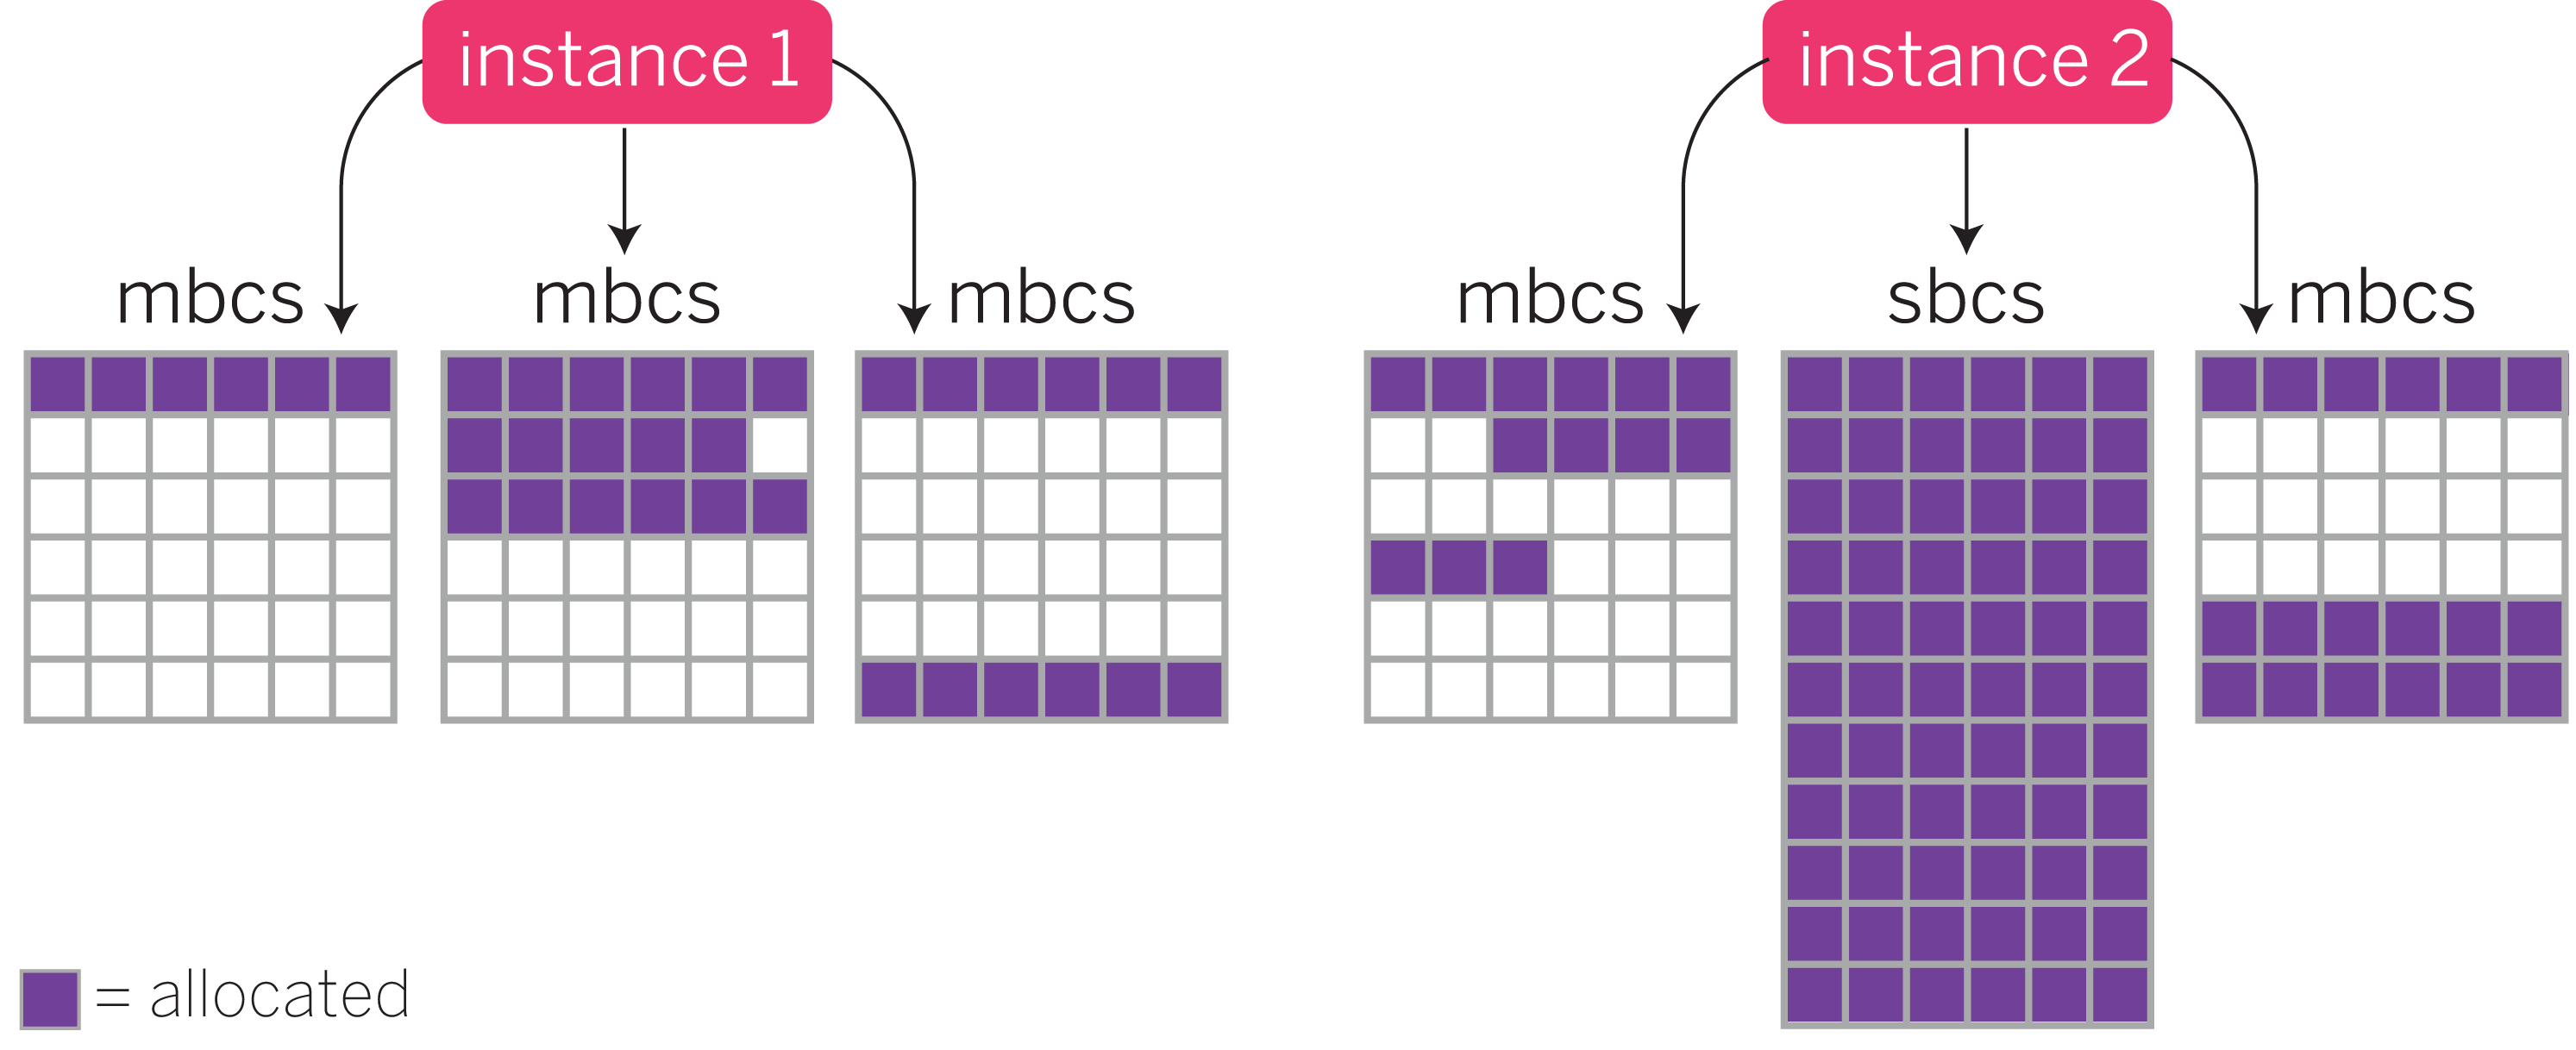
\includegraphics{allocation-1-normal.pdf}%
%  \caption{Example memory allocated in a specific sub-allocator}%
	\caption{Пример памяти, выделенной некоторым вложенным аллокатором}
   \label{fig:allocation-1-normal}
\end{figure}
\FloatBarrier

%Whenever a multiblock carrier (or the first \term{mmsbc}\footnote{\href{http://erlang.org/doc/man/erts\_alloc.html\#M\_mmsbc}{http://erlang.org/doc/man/erts\_alloc.html\#M\_mmsbc}} single block carriers) can be reclaimed, \term{mseg\_alloc} will try to keep it in memory for a while so that the next allocation spike that hits your VM can use pre-allocated memory rather than needing to ask the system for more each time.
Когда мультиблочный носитель (или первые \term{mmsbc}\footnote{\href{http://erlang.org/doc/man/erts\_alloc.html\#M\_mmsbc}{http://erlang.org/doc/man/erts\_alloc.html\#M\_mmsbc}} одноблочных носителей) могут быть возвращены операционной системе, \term{mseg\_alloc} попытается удержать их в памяти в течение некоторого времени на случай, если возникнет всплеск запросов выделения памяти, чтобы можно было взять готовые блоки, а не требовать создания новых.

%You then need to know the different memory allocation strategies of the Erlang virtual machine:
Затем вам нужно узнать о различных стратегиях выделения памяти, которые есть в виртуальной машине Erlang:

\begin{enumerate*}
%    \item Best fit (\term{bf})
	\item Best fit (\term{bf}) --- лучший подходящий размер.
%    \item Address order best fit (\term{aobf})
	\item Address order best fit (\term{aobf}) --- лучший подходящий в порядке адресов.
%    \item Address order first fit (\term{aoff})
	\item Address order first fit (\term{aoff}) --- первый подходящий в порядке адресов.
%    \item Address order first fit carrier best fit (\term{aoffcbf})
	\item Address order first fit carrier best fit (\term{aoffcbf}) --- первый подходящий в порядке адресов, лучший подходящий носитель.
%    \item Address order first fit carrier address order best fit (\term{aoffcaobf})
	\item Address order first fit carrier address order best fit (\term{aoffcaobf}) --- первый подходящий в порядке адресов, лучший подходящий носитель в порядке адресов.
%    \item Good fit (\term{gf})
	\item Good fit (\term{gf}) --- достаточно хорошо подходящий.
%    \item A fit (\term{af})
	\item A fit (\term{af}) -- какой попало подходящий.
\end{enumerate*}

%Each of these strategies can be configured individually for each \term{alloc\_util} allocator\footnote{\href{http://erlang.org/doc/man/erts\_alloc.html\#M\_as}{http://erlang.org/doc/man/erts\_alloc.html\#M\_as}}
Каждая из этих стратегий может быть настроена индивидуально для каждого аллокатора \term{alloc\_util}\footnote{\href{http://erlang.org/doc/man/erts\_alloc.html\#M\_as}{http://erlang.org/doc/man/erts\_alloc.html\#M\_as}}.

\begin{figure}
  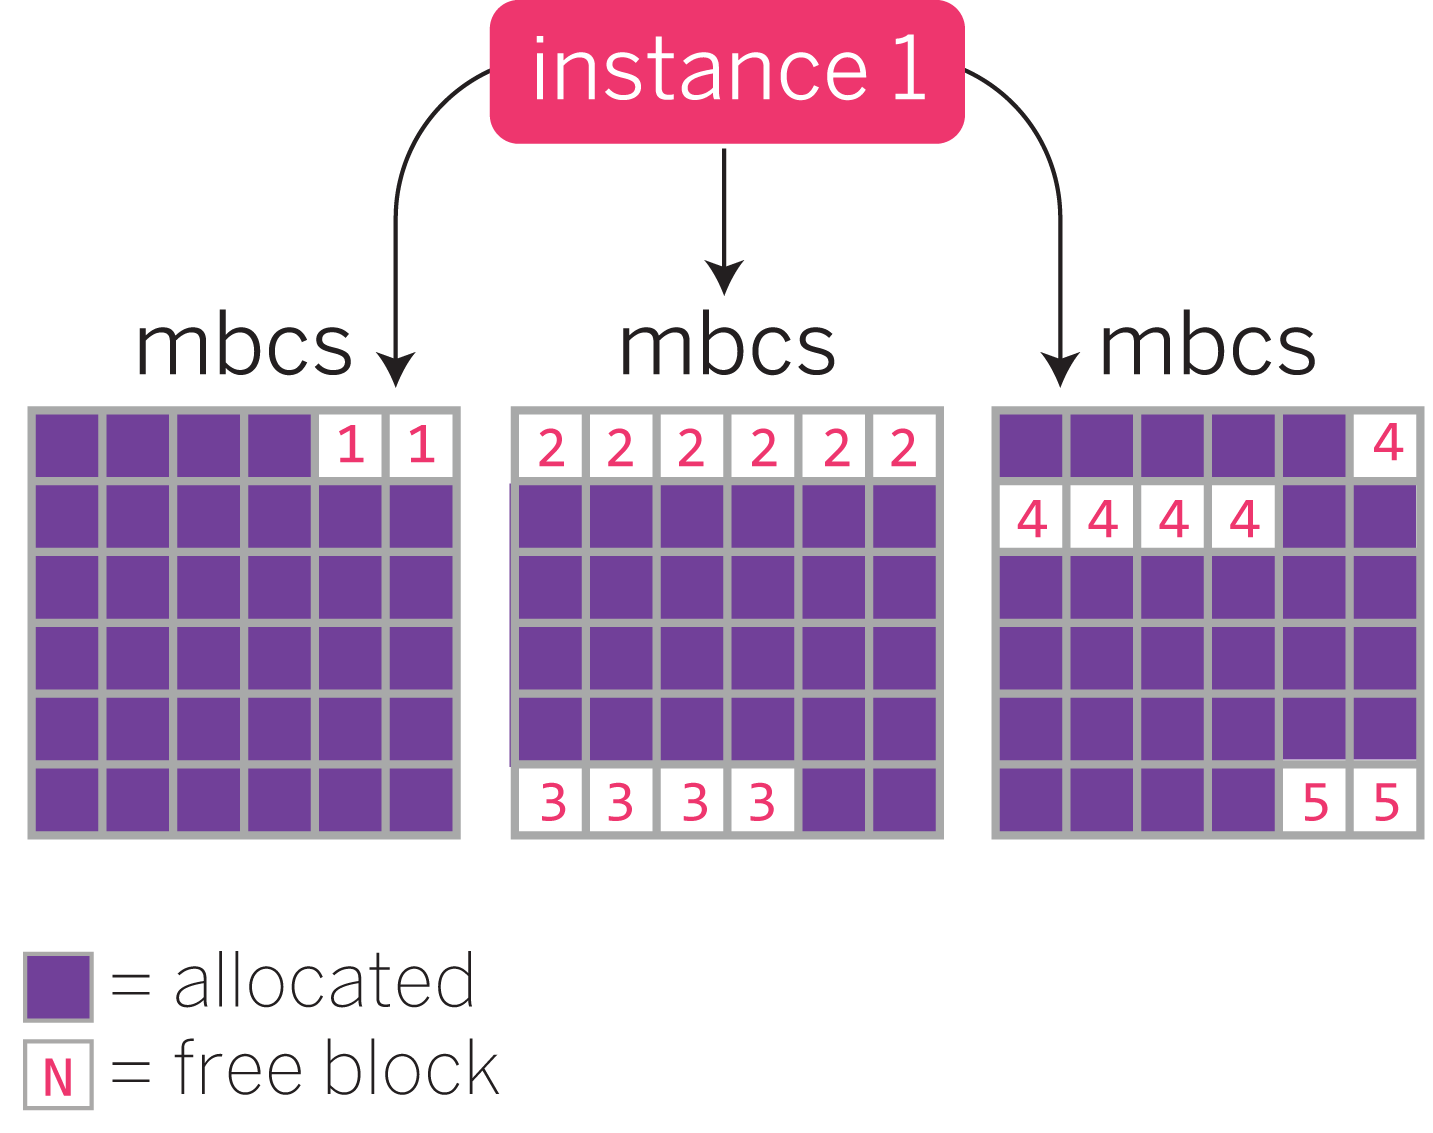
\includegraphics[max height=7cm]{allocation-strategy-1.pdf}%
  \centering%
%  \caption{Example memory allocated in a specific sub-allocator}%
	\caption{Пример памяти, выделенной некоторым вложенным аллокатором}
   \label{fig:allocation-strategy-1}
\end{figure}
\FloatBarrier

%For \emph{best fit} (\term{bf}), the VM builds a balanced binary tree of all the free blocks' sizes, and will try to find the smallest one that will accommodate the piece of data and allocate it there. In Figure \NamedRef{fig:allocation-strategy-1}, having a piece of data that requires three blocks would likely end in area 3.
Для стратегии \emph{best fit} (\term{bf}) виртуальная машина строит сбалансированное дерево, содержащее размеры всех свободных блоков и пытается найти наименьший подходящий свободный интервал и разместить блок в нём. На рисунке \ref{fig:allocation-strategy-1} при необходимости выделить блок данных длиной три клеточки, вероятнее всего он попадёт в область 3.

%\emph{Address order best fit} (\term{aobf}) will work similarly, but the tree instead is based on the addresses of the blocks. So the VM will look for the smallest block available that can accommodate the data, but if many of the same size exist, it will favor picking one that has a lower address. If I have a piece of data that requires three blocks, I'll still likely end up in area 3, but if I need two blocks, this strategy will favor the first \term{mbcs} in Figure \NamedRef{fig:allocation-strategy-1} with area 1 (instead of area 5). This could make the VM have a tendency to favor the same carriers for many allocations.
Стратегия \emph{Address order best fit} (\term{aobf}) будет работать подобным образом, но вместо этого дерево будет построено на основе адресов блоков. Так что виртуальная машина будет искать наименьший доступный блок, который может принять заданный размер данных, но если существуют несколько вариантов выбора, то будет предпочитать тот, у которого адрес меньше. Если у меня есть фрагмент данных, который требует два блока, то эта стратегия предпочтёт первый мультиноситель (\term{mbcs}) на рисунке \ref{fig:allocation-strategy-1} с номером 1 (вместо зоны под номером 5). Это даёт виртуальной машине склонность предпочитать одни и те же носители для множества распределений памяти.

%\emph{Address order first fit} (\term{aoff}) will favor the address order for its search, and as soon as a block fits, \term{aoff} uses it. Where \term{aobf} and bf would both have picked area 3 to allocate four blocks in Figure \NamedRef{fig:allocation-strategy-1}, this one will get area 2 as a first priority given its address is lowest. In Figure \NamedRef{fig:allocation-strategy-2}, if we were to allocate four blocks, we'd favor block 1 to block 3 because its address is lower, whereas \term{bf} would have picked either 3 or 4, and \term{aobf} would have picked 3.
\emph{Address order first fit} (\term{aoff}) будет руководствоваться порядком адресов при поиске, но как только найден первый подходящий блок, \term{aoff} его использует. В случае, когда стратегии \term{aobf} и \term{bf} использовали бы зону 3 для выделения четырёх блоков на рисунке \ref{fig:allocation-strategy-1}, эта стратегия выбрала бы зону 2, поскольку её адрес меньше. На рисунке  \ref{fig:allocation-strategy-2}, если бы нам понадобилось выделить четыре блока, мы бы предпочли блок 1 блоку 3, поскольку его адрес меньше, тогда как \term{bf} выбрал бы вариант 3 или 4, а \term{aobf} выбрал бы 3.

\begin{figure}
  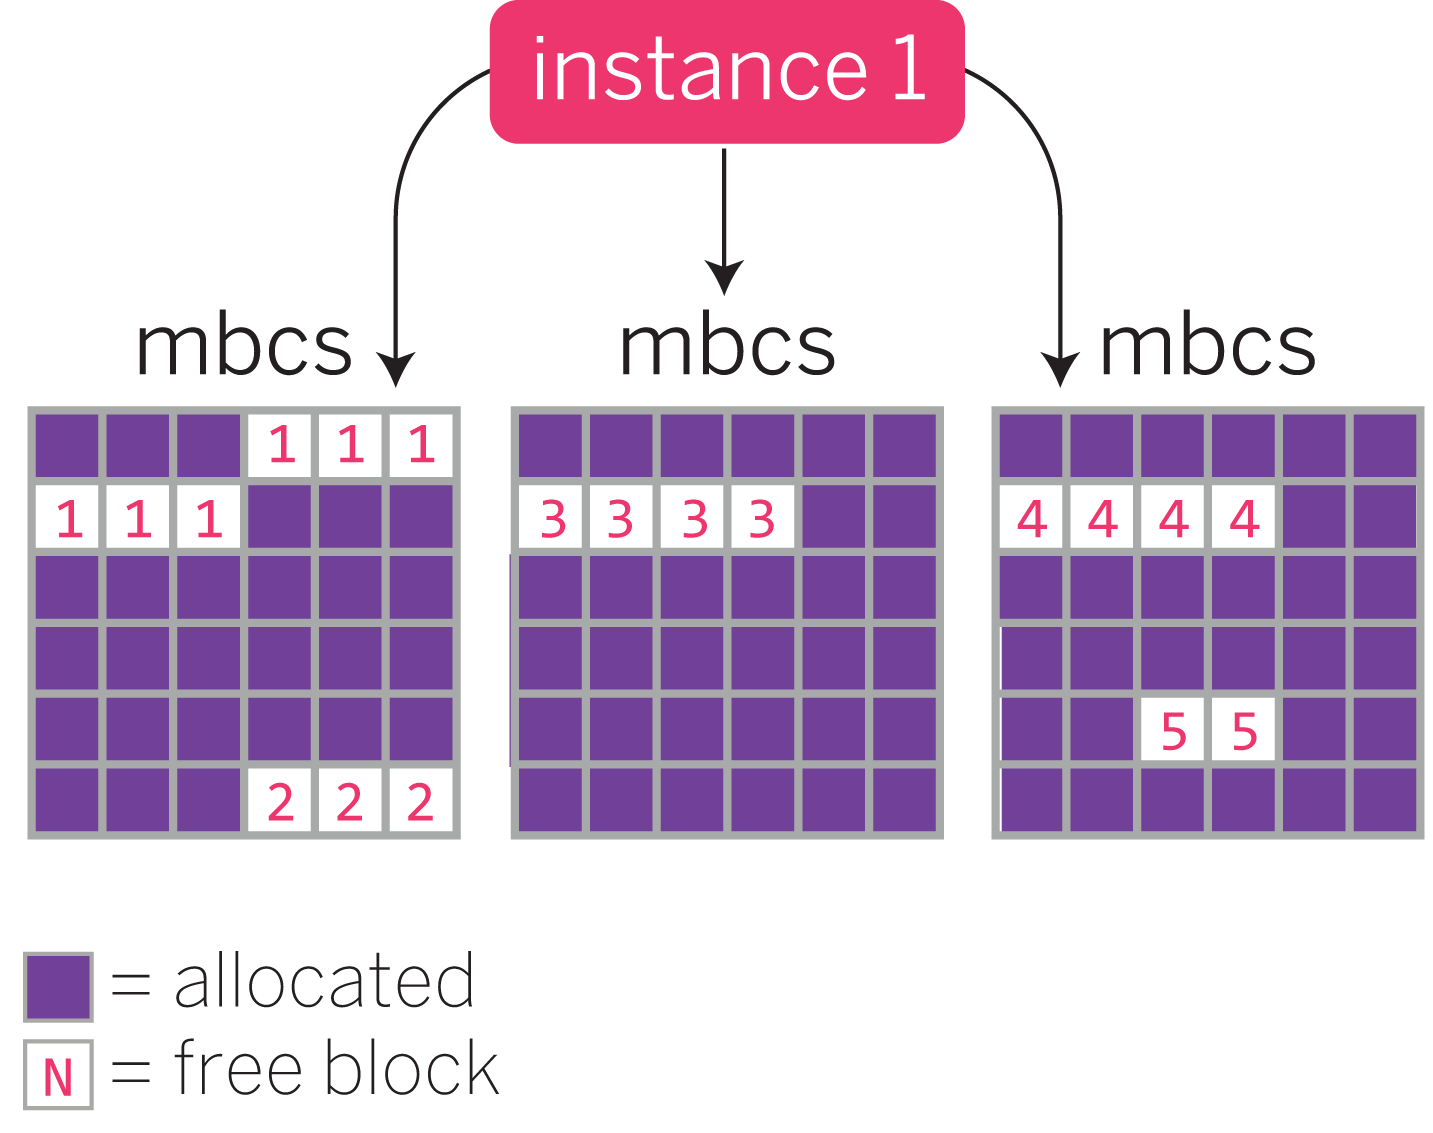
\includegraphics[max height=7cm]{allocation-strategy-2.pdf}%
  \centering%
%  \caption{Example memory allocated in a specific sub-allocator}%
	\caption{Пример памяти, выделенной некоторым вложенным аллокатором}
   \label{fig:allocation-strategy-2}
\end{figure}
\FloatBarrier

%\emph{Address order first fit carrier best fit} (\term{aoffcbf}) is a strategy that will first favor a carrier that can accommodate the size and then look for the best fit within that one. So if we were to allocate two blocks in Figure \NamedRef{fig:allocation-strategy-2}, \term{bf} and \term{aobf} would both favor block 5, \term{aoff} would pick block 1. \term{aoffcbf} would pick area 2, because the first \term{mbcs} can accommodate it fine, and area 2 fits it better than area 1.
\emph{Address order first fit carrier best fit} (\term{aoffcbf}) --- это стратегия, отдающая предпочтение носителю, который сможет принять нужный размер блока и затем в выбранном носителе выполняется поиск по лучшему подходящему размеру. Итак, если бы нам нужно было выделить два блока на рисунке \ref{fig:allocation-strategy-2}, то стратегии \term{bf} и \term{aobf} отдали бы предпочтение зоне 5, \term{aoff} выбрала бы блок 1. \term{aoffcbf} выбрала бы зону 2, поскольку первый мультиноситель (\term{mbcs}) может принять его, и зона 2 подходит лучше зоны 1.

%\emph{Address order first fit carrier address order best fit} (\term{aoffcaobf}) will be similar to \term{aoffcbf}, but if multiple areas within a carrier have the same size, it will favor the one with the smallest address between the two rather than leaving it unspecified.
\emph{Address order first fit carrier address order best fit} (\term{aoffcaobf}) ведёт себя подобно \term{aoffcbf}, но если внутри носитепля есть множество зон одинакового размера, он отдаст предпочтение той, у которой адрес наименьший вместо того, чтоб выбирать по какой-то своей неназванной логике.

%\emph{Good fit} (\term{gf}) is a different kind of allocator; it will try to work like best fit (\term{bf}), but will only search for a limited amount of time. If it doesn't find a perfect fit there and then, it will pick the best one encountered so far. The value is configurable through the \term{mbsd}\footnote{\href{http://www.erlang.org/doc/man/erts\_alloc.html\#M\_mbsd}{http://www.erlang.org/doc/man/erts\_alloc.html\#M\_mbsd}} VM argument.
\emph{Good fit} (\term{gf}) --- попытается сработать аналогично \emph{best fit} (\term{bf}), но будет выполнять поиск только в течение ограниченного времени. Если не удалось за это время найти хорошо подходящий блок, тогда он выберет лучший найденный до сих пор. Значение можно настроить параметром \term{mbsd}\footnote{\href{http://www.erlang.org/doc/man/erts\_alloc.html\#M\_mbsd}{http://www.erlang.org/doc/man/erts\_alloc.html\#M\_mbsd}} виртуальной машины.

%\emph{A fit} (\term{af}), finally, is an allocator behaviour for temporary data that looks for a single existing memory block, and if the data can fit, \term{af} uses it. If the data can't fit, \term{af} allocates a new one.
И наконец, \emph{A fit} (\term{af}), поведение аллокатора для временных данных, которое ищет единственный блок памяти, в который могут поместиться данные, и использует его. Если данные не помещаются --- то \term{af} выделит новый.

%Each of these strategies can be applied individually to every kind of allocator, so that the heap allocator and the binary allocator do not necessarily share the same strategy.
Каждая из этих стратегий может быть назначена индивидуально к каждому типу аллокаторов, так что аллокаторы кучи и двоичных данных могут вполне иметь разные стратегии.

%Finally, starting with Erlang version 17.0, each \term{alloc\_util} allocator on each scheduler has what is called a \emph{\term{mbcs} pool}. The \term{mbcs} pool is a feature used to fight against memory fragmentation on the VM. When an allocator gets to have one of its multiblock carriers become mostly empty,\footnote{The threshold is configurable through \href{http://www.erlang.org/doc/man/erts\_alloc.html\#M\_acul}{http://www.erlang.org/doc/man/erts\_alloc.html\#M\_acul}} the carrier becomes \emph{abandoned}. 
Начиная с версии Erlang 17.0, каждый аллокатор \term{alloc\_util} на каждом планировщике имеет некий так называемый пул мультиблочных носителей \emph{\term{mbcs} pool}. Это возможность, используемая для борьбы с фрагментацией памяти на виртуальной машине. Когда один из мультиблочных носителей аллокатора почти опустошается,\footnote{Порог срабатывания можно настроить \href{http://www.erlang.org/doc/man/erts\_alloc.html\#M\_acul}{http://www.erlang.org/doc/man/erts\_alloc.html\#M\_acul}}, то носитель становится \emph{брошенным}.

%This abandoned carrier will stop being used for new allocations, until new multiblock carriers start being required. When this happens, the carrier will be fetched from the \term{mbcs} pool. This can be done across multiple \term{alloc\_util} allocators of the same type across schedulers. This allows the VM to cache mostly-empty carriers without forcing deallocation of their memory.\footnote{In cases this consumes too much memory, the feature can be disabled with the options \term{+MBacul 0}.} It also enables the migration of carriers across schedulers when they contain little data, according to their needs.
Такой брошенный носитель прекращает использоваться для новых распределений памяти до тех пор, пока не начнут требоваться новые мультиблочные носители. Когда это случается, носитель извлекается из пула \term{mbcs}. Это может произойти в разных аллокаторах \term{alloc\_util} одного и того же типа, на любом планировщике задач. Это позволяет виртуальной машине сохранить почти пустые носители не заставляя их освободить остатки памяти\footnote{Если оказывается так, что это приводит к большому расходу памяти, возможность можно отключить опцией \term{+MBacul 0}.}. Также это позволяет миграцию носителей, содержащих немного данных, между планировщиками по необходимости.


%\subsubsection{The Process Level}
\subsubsection{Взгляд на уровне процесса}
\label{subsec:memory-process-level}

%On a smaller scale, for each Erlang process, the layout still is a bit different. It basically has this piece of memory that can be imagined as one box:
В меньшем масштабе, для каждого процесса Erlang, устройство памяти немного отличается. Можно представить себе некий контейнер, являющийся блоком в памяти, изобразим его так:

\begin{VerbatimText}
[                  ]
\end{VerbatimText}

%On one end you have the heap, and on the other, you have the stack:
В одном конце его находится куча, а в другом --- стек:

\begin{VerbatimText}
[куча |      | стек]
\end{VerbatimText}

%In practice there's more data (you have an old heap and a new heap, for generational GC, and also a virtual binary heap, to account for the space of reference-counted binaries on a specific sub-allocator not used by the process — \term{binary\_alloc} vs. \term{eheap\_alloc}):
На практике данных больше (есть старая куча, и новая куча, для сборщика мусора, работающего с поколениями памяти, а также куча для двоичных данных, чтобы с их помощью считать ссылки на большие двоичные данные в большой куче, отдельно от процесса --- \term{binary\_alloc} против \term{eheap\_alloc}):

\begin{VerbatimText}
[куча   ||     стек]
\end{VerbatimText}

%The space is allocated more and more up until either the stack or the heap can't fit in anymore. This triggers a minor GC. The minor GC moves the data that can be kept into the old heap. It then collects the rest, and may end up reallocating more space.
Место продолжает выделяться с двух концов до тех пор, пока стек или куча не перестают помещаться. Это включает малый цикл сборки мусора. Эта сборка перемещает данные, которые продолжают существовать, в старую кучу. Затем сборщик собирает то, что осталось и, возможно, выделит новый блок памяти большего размера.

%After a given number of minor GCs and/or reallocations, a full-sweep GC is performed, which inspects both the new and old heaps, frees up more space, and so on. When a process dies, both the stack and heap are taken out at once. reference-counted binaries are decreased, and if the counter is at 0, they vanish.
После заданного количества малых сборок мусора и перевыделений новой памяти, выполняется полный цикл сборки мусора (\emph{full-sweep}), который анализирует новую и старую кучи, освобождает дополнительное место и так далее. Когда процесс умирает, стек и куча одновременно освобождаются, уменьшаются счётчики на двоичных данных, которые хранятся по количеству ссылок, и если они достигают нуля, то данные тоже освобождаются.

%When that happens, over 80\% of the time, the only thing that happens is that the memory is marked as available in the sub-allocator and can be taken back by new processes or other ones that may need to be resized. Only after having this memory unused — and the multiblock carrier unused also — is it returned to \term{mseg\_alloc} or \term{sys\_alloc}, which may or may not keep it for a while longer.
Когда это происходит, то в 80\% случаях память оказывается отмеченной во вложенном аллокаторе, как свободная, и может быть взята новыми или другими процессами, которым потребовалось изменение размера. Только после того, как эта память не была использована в течение некоторого времени --- и мультиблочный носитель не был использован тоже --- память будет возвращена системному аллокатору, откуда она была взята (\term{mseg\_alloc} или \term{sys\_alloc}), который на своё усмотрение может удержать её ещё некоторое время.


%\subsection{Fixing Memory Fragmentation with a Different Allocation Strategy}
\subsection{Боремся с фрагментацией, изменяя стратегию распределения памяти}

%Tweaking your VM's options for memory allocation may help.
Можно попробовать настроить параметры виртуальной машины, отвечающие за распределение памяти.

%You will likely need to have a good understanding of what your type of memory load and usage is, and be ready to do a lot of in-depth testing. The \module{recon\_alloc} module contains a few helper functions to provide guidance, and the module's documentation\footnote{\href{http://ferd.github.io/recon/recon\_alloc.html}{http://ferd.github.io/recon/recon\_alloc.html}} should be read at this point.
Вероятно вам понадобится хорошее понимание вашей ситуации с нагрузкой на память и её использованием, и будьте готовы провести множество тестов для выяснения этих фактов. Модуль \module{recon\_alloc} содержит несколько вспомогательных функций, которые направят ваш путь, и это будет самым подходящим временем прочесть документацию к модулю\footnote{\href{http://ferd.github.io/recon/recon\_alloc.html}{http://ferd.github.io/recon/recon\_alloc.html}}.

%You will need to figure out what the average data size is, the frequency of allocation and deallocation, whether the data fits in \term{mbcs} or \term{sbcs},  and you will then need to try playing with a bunch of the options mentioned in \module{recon\_alloc}, try the different strategies, deploy them, and see if things improve or if they impact times negatively.
Вам нужно будет выяснить средний размер ваших данных в памяти, частоту распределений и освобождений, попадают ли ваши данные в мультиблоки (\term{mbcs}) или в одиночные блоки (\term{sbcs}), и затем попробуйте поиграть с множеством опций, которые упомянуты в модуле \module{recon\_alloc}. Попробуйте разные стратегии, установите их, сравните ситуацию --- улучшилась ли она или всё стало медленнее и хуже.

%This is a very long process for which there is no shortcut, and if issues happen only every few months per node, you may be in for the long haul. 
Это долгий кропотливый процесс для которого нет известного короткого пути, и если проблемы случаются каждые несколько месяцев, то будьте готовы к тому, что поиски затянутся.


\section{Упражнения}

\subsection*{\ReviewTitle{}}

\begin{enumerate}
%	\item Name some of the common sources of leaks in Erlang programs.
	\item Назовите несколько известных вам источников утечек ресурсов в Erlang-программах.
%	\item What are the two main types of binaries in Erlang?
	\item Какие два вида блоков двоичных данных имеются в Erlang?
%	\item What could be to blame if no specific data type seems to be the source of a leak?
	\item Где следует искать, если никакой из типов данных не выглядит источником утечки?
%	\item If you find the node died with a process having a lot of memory, what could you do to find out which one it was?
	\item Если вы обнаружили смерть узла, в котором один из процессов занял очень много памяти, что вы можете сделать для поиска виновного процесса?
%	\item How could code itself cause a leak?
	\item Как сам код может явиться причиной утечки?
%	\item How can you find out if garbage collections are taking too long to run?
	\item Как можно выяснить, что сборка мусора начала занимать очень долгое время?
\end{enumerate}

\subsection*{\OpenEndedTitle{}}

\begin{enumerate}
%	\item  How could you verify if a leak is caused by forgetting to kill processes, or by processes using too much memory on their own?
	\item Как можно проверить, является ли причиной утечки то, что вы забыли убить ненужные процессы или они просто сами начали использовать слишком много памяти?
%	\item A process opens a 150MB log file in binary mode to go extract a piece of information from it, and then stores that information in an ETS table. After figuring out you have a binary memory leak, what should be done to minimize binary memory usage on the node?
	\item Некий процесс открывает 150-мегабайтовый файл журнала в режиме двоичного чтения для извлечения некоторой информации, затем сохраняет информацию в ETS-таблице. После выяснения наличия у вас утечки двоичной памяти, что можно сделать, чтобы минимизировать расход двоичной памяти на данном узле?
%	\item What could you use to find out if ETS tables are growing too fast?
	\item Что можно использовать для выяснения того факла, что ваши ETS-таблицы растут слишком быстро?
%	\item What steps should you go through to find out that a node is likely suffering from fragmentation? How could you disprove the idea that is could be due to a NIF or driver leaking memory?
	\item Какие шаги вам следует пройти, чтобы узнать, что ваш узел вероятно страдает от фрагментации памяти? Как можно опровергнуть догадку, что виновником мог являться драйвер или встроенная (NIF) функция?
%	\item How could you find out if a process with a large mailbox (from reading \term{message\_queue\_len}) seems to be leaking data from there, or never handling new messages?
	\item Как можно выяснить, что процесс с большим почтовым ящиком (посредством чтения параметра \term{message\_queue\_len}) вероятно имеет утечку памяти из ящика или не обслуживает новые сообщения?
%	\item A process with a large memory footprint seems to be rarely running garbage collections. What could explain this?
	\item Процесс с большим потреблением памяти вероятно редко выполняет сборку мусора. Чем можно это объяснить?
%	\item When should you alter the allocation strategies on your nodes? Should you prefer to tweak this, or the way you wrote code?
	\item Когда вам следует изменять стратегии распределения памяти на ваших узлах? Предпочтёте ли вы настраивать стратегии или исправить ваш код?
\end{enumerate}

\subsection*{\HandsOnTitle{}}

\begin{enumerate}
%	\item Using any system you know or have to maintain in Erlang (including toy systems), can you figure out if there are any binary memory leaks on there?
	\item Используя любую систему, которая вам знакома или которую вам приходится обслуживать, написанную на Erlang (включая игрушечные системы для незначительных проектов), сможете ли вы выяснить, имеет ли эта система утечки двоичной памяти?
\end{enumerate}
	
%%%
%%%
%%%

%%% Cognitive
%%
%% These should be done after reading the standard documentation on crash dumps referenced by the text.
%%
%% Knowledge: recall facts, terms, basic concepts
%% 
%% - What are the two main ways to find about a memory leak?
%% - What are good questions to ask about the node if you suspect a leak?
%% - Name some of the common sources of leaks in Erlang programs.
%% - What are the two main types of binaries in Erlang?
%% - What could be to blame if no specific data type seems guilty of a leak?
%% - Can Erlang's memory allocation schemes be modified or are they unchangeable without patches?
%%
%% Comprehension: organizing, comparing, translating, interpreting, giving descriptions, and stating the main ideas
%%
%% - How could you verify if a leak is caused by forgetting to kill processes, or by processes using too much memory on their own?
%% - What could cause the atom table to grow infinitely?
%% - How could code itself cause a leak?
%% - How can you find out if garbage collections are taking too long to run?
%%
%% Application: Solve problems in new situations by applying acquired knowledge, facts, techniques and rules in a different way
%%
%% - Using any system you know or have to maintain in Erlang (including toy systems), can you figure out if there are any binary memory leaks on there?
%% - A process opens a 150MB log file in binary mode to go extract a piece of information from it, and then stores that information in an ETS table. After figuring out you have a binary memory leak, what should be done to minimize binary memory usage on the node?
%% - What could you use to find out if ETS tables are growing too fast?
%%
%% Analysis: break down info, make inferences, find evidence
%%
%% - What steps should you go through to find out that a node is likely suffering from fragmentation? How could you disprove the idea that is could be due to a NIF or driver leaking memory?
%%
%% Synthesis: Compile information together in a different way by combining elements in a new pattern or proposing alternative solutions
%%
%% - How could you find out if a process with a large mailbox (from reading 'message_queue_len') seems to be leaking data from there, or never handling new messages?
%% - A process with a large memory footprint seems to be rarely running garbage collections. What could explain this?
%%
%% Evaluation: Present and defend opinions by making judgments about information
%%
%% - When should you alter the allocation strategies on your nodes? Should you prefer to tweak this, or the way you wrote code?
%% 
